\chapter{Calculating congruence lattices}
\label{chap:lattice}

We can learn a lot about a semigroup's structure by examining its congruences:
they describe a semigroup's homomorphic images, and quotient semigroups, as
explained in Section \ref{sec:intro-congs}.  For this reason, it is of great
interest to be able to produce a complete list of congruences on a given
semigroup.

In group theory, we study normal subgroups instead of studying congruences
directly (see Section \ref{sec:normal-subgroups}).  Several algorithms exist for
computing a given group's normal subgroups, and therefore its congruences.  We
will briefly outline the approach used in GAP, referring the reader to
\cite{hulpke_1998} for a fuller explanation.  To compute the normal subgroups of
a group $G$, we first compute a \textit{chief series} for $G$---that is, a
series of $k$ normal subgroups of $G$,
\index{chief series}
$$1 = N_k
\triangleleft N_{k-1}
\triangleleft \ldots
\triangleleft N_1
\triangleleft N_0 = G,$$
such that there exists no normal subgroup $A \trianglelefteq G$ with
$N_i \triangleleft A \triangleleft N_{i-1}$ for any $i \in \{1, \ldots, k\}$.
Once such a chief series has been computed, the normal subgroups of $G / N_i$
are computed inductively along the series: $G / N_0$ is trivial, and at each
subsequent step we compute the normal subgroups of $G / N_i$ using the normal
subgroups of $G / N_{i-1}$, until on the last step we have the normal subgroups
of $G / N_k = G$.  Unfortunately, this method is not applicable to arbitrary
semigroups, since semigroup theory has no concept equivalent to that of a chief
series to which we might apply the algorithm.  Hence, we must seek an
alternative approach to apply to semigroups more generally.

In this chapter, we present a method for calculating all the congruences of a
finite semigroup.  This algorithm takes advantage of the fact that congruences
lie in a lattice with respect to containment ($\subseteq$), intersection
($\cap$) and join ($\vee$).  It computes the lattice structure while it computes
the congruences themselves, and so the lattice structure is returned as an
output of the algorithm, along with the set of congruences.  This algorithm was
used as a starting point for the work described in Chapter \ref{chap:motzkin}.

In Section \ref{sec:lattice-algorithm} we give the algorithm in pseudo-code, and
explain how it works.  In Section \ref{sec:lattice-implementation} we outline
some practical concerns for implementing the algorithm, with particular
reference to how it is implemented in the Semigroups package \cite{semigroups}
for GAP \cite{gap}.  And finally, in Section \ref{sec:lattice-examples}, we
present some examples of lattices which have been computed using this algorithm.

\section{The algorithm}
\label{sec:lattice-algorithm}

For the purposes of this section, we will make the following definition.

\begin{definition}
  \label{def:congruence-poset}
  \index{congruence!poset}
  A \textbf{congruence poset} on a semigroup $S$ is a pair $(\Gamma, \PO)$
  where:
  \begin{itemize}
  \item $\Gamma$ is a set of congruences on $S$; and
  \item $\PO$ is $\subseteq$, the partial order of containment on $\Gamma$.
  \end{itemize}
\end{definition}

Recall that a partial order is defined as a relation that is reflexive
($x \leq x$), anti-symmetric ($x \leq y$ and $y \leq x$ if and only if $x = y$),
and transitive ($x \leq y$ and $y \leq z$ implies $x \leq z$).
\index{partial order}
Hence $\PO$ will be a set of pairs of the form $(\rho, \sigma)$, where $\rho$
and $\sigma$ are both congruences on $S$, and $\rho \subseteq \sigma$.  If
$\Gamma$ is the set of all congruences on $S$, then $(\Gamma, \PO)$ will be a
lattice by Theorem \ref{thm:congruence-lattice}, and two congruences $\rho$ and
$\sigma$ will have an intersection $\rho \cap \sigma$ and a join
$\rho \vee \sigma$ in $\Gamma$.  But note that in general, a congruence poset
need not be closed under such operations.

\subsection{Principal congruences}
\label{sec:princ-cong-poset}

We first present an algorithm to calculate the principal congruences of a
semigroup, along with their partial ordering $\subseteq$.  This is a congruence
poset, but since it may not contain all the congruences on the given semigroup,
it may not be a lattice.  We call this algorithm \textsc{PrincCongPoset}.
Pseudo-code for is given for it in Algorithm \ref{alg:princ-cong-poset}, and it
is discussed in more detail below.

\begin{algorithm}
  \caption{The \textsc{PrincCongPoset} algorithm}
  \label{alg:princ-cong-poset}
  \index{PrincCongPoset@\textsc{PrincCongPoset}}
  \begin{algorithmic}[1]
    \Require $S$ a finite semigroup
    \Procedure{PrincCongPoset}{$S$}
      \State $\Gamma := \varnothing$
      \Comment{Set of congruences}
      \State $\PO := \varnothing$
      \Comment{Partial order ($\subseteq$) on congruences}
      \For{$(x,y) \in S \times S$} \label{line:for-x-y}
        \State $P := \left\{\big((x,y)^\sharp, (x,y)^\sharp\big)\right\}$
        \Comment{$(x,y)^\sharp \subseteq (x,y)^\sharp$}
        \For{$(a,b)^\sharp \in \Gamma$}
          \If{$(x,y) \in (a,b)^\sharp$}
            \If{$(a,b) \in (x,y)^\sharp$}
              \State \Goto line \ref{line:for-x-y} and next pair $(x,y)$
              \Comment{$(a,b)^\sharp = (x,y)^\sharp$}
            \Else
              \State $P \gets P \cup
                \left\{\big((x,y)^\sharp, (a,b)^\sharp\big)\right\}$
                \Comment{$(x,y)^\sharp \subseteq (a,b)^\sharp$}
            \EndIf
          \ElsIf{$(a,b) \in (x,y)^\sharp$}
              \State $P \gets P \cup
                \left\{\big((a,b)^\sharp, (x,y)^\sharp\big)\right\}$
                \Comment{$(a,b)^\sharp \subseteq (x,y)^\sharp$}
          \EndIf
        \EndFor
        \State $\Gamma \gets \Gamma \cup \{(x,y)^\sharp\}$
        \State $\PO \gets \PO \cup P$
        % \State Add $(x,y)^\sharp \leq (a,b)^\sharp$ for each $(a,b)^\sharp$ in $P$
        % \State Add $(a,b)^\sharp \leq (x,y)^\sharp$ for each $(a,b)^\sharp$ in $C$
        % \For{$(a,b)^\sharp \in P$}
        %   \State Set $(x,y)^\sharp \leq (a,b)^\sharp$
        % \EndFor
        % \For{$(a,b)^\sharp \in C$}
        %   \State Set $(a,b)^\sharp \leq (x,y)^\sharp$
        % \EndFor
        % \State $\PO \gets \PO \cup
        % \big\{\big((x,y)^\sharp, (a,b)^\sharp\big) : (a,b)^\sharp \in P\big\}$
        % \State $\PO \gets \PO \cup
        % \big\{\big((a,b)^\sharp, (x,y)^\sharp\big) : (a,b)^\sharp \in C\big\}$
      \EndFor
      \State \Return $(\Gamma, \PO)$
    \EndProcedure
  \end{algorithmic}
\end{algorithm}

The \textsc{PrincCongPoset} algorithm is not a very sophisticated algorithm,
being based on a concept with a lot of brute-force work checking the presence of
pairs in a congruence.  However, when paired with the fast code in
\texttt{libsemigroups} \cite{libsemigroups} for testing the presence of a pair
in a single congruence (as described in Chapter \ref{chap:pairs}) it can give
results about small semigroups in a reasonable amount of time.

The idea of the algorithm is to go through each pair in $S \times S$, and
consider the congruence generated by that pair.  We compare each new congruence
to the congruences we have found so far, establishing which of them it contains,
and which it is contained in.  If it turns out to be equal to a congruence
already found, we drop it immediately; if it turns out to be an entirely new
congruence, then we can add it to the list $\Gamma$ of congruences, and add
pairs to $\PO$ that describe how it compares to the other congruences.  Since
each new congruence is compared to every previously found congruence, every
possible appropriate pair is added to $\PO$, and we are therefore guaranteed
that $\PO$ will be equal to the containment relation ($\subseteq$) by the end of
the algorithm.

One positive outcome of using generating pairs in this way is that we can use
the result
$$(a,b)^\sharp \subseteq (x,y)^\sharp \quad\iff\quad (a,b) \in (x,y)^\sharp$$
for any two pairs $(a,b), (x,y) \in S \times S$.  Hence, in order to compare the
two congruences comprehensively, we only need to test the presence of one pair
in each congruence: $(a,b) \in (x,y)^\sharp$ and $(x,y) \in (a,b)^\sharp$.
Testing the presence of a given pair in a congruence is likely to be faster
than, for example, exhaustively computing its congruence classes.  A general
algorithm for testing whether a given pair lies in a congruence specified by
generating pairs is described in Chapter \ref{chap:pairs}; in some cases this
can be improved by first converting the congruence to another representation, as
described in Chapter \ref{chap:converting}.

Since this algorithm is based on iterating over all the pairs in $S \times S$,
the time taken to compute the principle congruences increases rapidly as $|S|$
grows.  This makes the algorithm ineffective for large semigroups.  However,
useful results can be obtained for small semigroups; see Section
\ref{sec:lattice-examples} for some examples.

Algorithm \ref{alg:princ-cong-poset} shows a theoretical description of the
\textsc{PrincCongPoset} algorithm, described in a fairly simple way to aid the
understanding of the reader.  However, it can be modified in a few simple ways
to improve its performance.  Firstly, we should consider the source of
generating pairs: we iterate through all pairs $(x,y) \in S \times S$.  There
are ways in which this process is guaranteed to encounter a given congruence
twice, and therefore waste time.  For example, if we consider a pair $(x,y)$,
there is no need later to consider $(y,x)$, since it will generate the same
congruence.  Similarly there is no need to consider every reflexive pair
$(x,x)$, since each one is guaranteed to generate the trivial congruence.  Thus,
if $S$ has $n$ elements, we need only consider $\frac{1}{2}n(n-1)$ pairs, rather
than all $n^2$ pairs from $S \times S$.  In the best cases, this may reduce the
runtime of the algorithm by more than 50\%; however, note that the complexity of
the algorithm is not improved.

Note that we could also replace $S$ here with some subset $X \subset S$, if we
wish to see what congruences can be generated only with pairs from $X \times X$.
For instance, we might be interested in congruences generated by pairs from some
ideal of $S$, and how they affect elements outside the ideal.  These questions
can be answered with minimal changes to the algorithm.

Another possible improvement would be to use pairs already in $\PO$, along with
the axiom of transitivity, to skip certain comparisons.  For example, if our new
congruence $(x,y)^\sharp$ is found to be a subset of $(a,b)^\sharp$, but
$(a,b)^\sharp$ is itself already known to be a subset of some congruence
$(c,d)^\sharp$, then we can immediately add the pair
$\big((x,y)^\sharp, (c,d)^\sharp\big)$ to $P$ and we can skip the comparison of
$(x,y)^\sharp$ to $(c,d)^\sharp$ later in the algorithm.  Since most of the
computational work in this algorithm tends to be in comparing congruences to
each other, this ability to skip comparisons is important.

\subsection{Adding joins}
\label{sec:join-closure}

\index{JoinClosure@\textsc{JoinClosure}}
Our second algorithm is called \textsc{JoinClosure}.  This algorithm takes a
congruence poset $(\Gamma, \PO)$ as its argument, and returns the congruence
poset containing all the congruences in $\Gamma$ along with all their joins.
That is, for any collection of $k$ congruences
$(\rho_i)_{1 \leq i \leq k}$ from $\Gamma$, the output of
\textsc{JoinClosure} will contain the congruence
$$\bigvee_{1 \leq i \leq k} \rho_i
\quad=\quad \rho_1 \vee \rho_2 \vee \ldots \vee \rho_k.$$

In order to calculate this, we can take advantage of one important property of
all lattices: a lattice can be viewed as a semigroup in its own right.  In
particular, the set of congruences of a semigroup forms a semigroup under the
operation $\vee$ of taking joins.  Hence, finding the join-closure of a
congruence poset $(\Gamma, \PO)$ is equivalent to finding the elements of the
semigroup generated by $\Gamma$ under $\vee$, along with information about how
they multiply together.

There exist several algorithms which compute all the elements of a semigroup $S$
using its generators $X$.  An overview of such algorithms can be found in
\cite[\S1]{computing_finite_semigroups}.  A relatively na\"ive algorithm would
simply create a list of elements, starting with the generators $X$, and multiply
each element in the list with each generator, on the right and left, adding any
new elements to the list and multiplying them in turn, until no new elements can
be found.  However, this algorithm would entail many unnecessary multiplications
that could be avoided by using a more sophisticated algorithm.  A better
candidate is the Froidure--Pin algorithm which was mentioned in Section
\ref{sec:find-pres}.  This algorithm, first described in \cite{froidure_pin},
takes a set of generators $X$ for a semigroup $S$ and returns, among other
things, left and right Cayley graphs for $S$, and a list of words $w \in X^+$
representing one possible factorisation of each $s \in S$ in terms of the
generators.  Naturally, this algorithm only works when the multiplication of
elements is well-defined and understood without knowledge of the semigroup as a
whole; fortunately, this is the case for the join operation $\vee$ on
congruences.

The outputs of the Froidure--Pin algorithm are sufficient to build up the entire
congruence lattice of a semigroup, given the principal congruences.  For each
congruence $\rho$ we have a word $w \in \Gamma^+$ representing how it is
factorised in terms of the generators: this factorisation is precisely a list of
principal congruences which need to be joined together to give $\rho$, which
gives us a list of pairs from $S \times S$ which generates the congruence.  The
right Cayley graph returned by the algorithm describes the lattice structure in
terms of joins ($\vee$), from which we can easily deduce the structure in terms
of containment ($\subseteq$).  Note that the left Cayley graph will be identical
to the right Cayley graph, since the lattice is commutative.  Again, a full
description of the Froidure--Pin algorithm is outside the scope of this thesis,
but it is described more completely in \cite{froidure_pin}, and the version
implemented in \texttt{libsemigroups} is explained in
\cite{froidure_pin_jonusas}.

The Froidure--Pin algorithm requires a method of deciding whether two
congruences are equal.  In \textsc{JoinClosure}, unlike in
\textsc{PrincCongPoset}, we may encounter congruences with more than one
generating pair.  Hence, for two congruences $\rho$ and $\sigma$, we cannot find
out whether $\rho = \sigma$ in quite the same way as we did in
\textsc{PrincCongPoset}.  However, we have one useful result: if $\mathbf{R}$
and $\mathbf{S}$ are sets of generating pairs, then
$$\Rs = \mathbf{S}^\sharp \quad\iff\quad
\R \subseteq \mathbf{S}^\sharp \textnormal{~and~}
\mathbf{S} \subseteq \Rs,$$
so we only have to check containment of generating pairs in order to check
equality of congruences.  However, a congruence may have many generating pairs,
so in some cases this check may take a long time.  For this reason, if there is
an alternative way of representing the congruences (for example, another
representation from Chapter \ref{chap:converting}) then it may be quicker to use
a containment method specific to that representation.  For example, if $S$ is a
0-simple semigroup, then our two congruences will have linked triples
$(N_1,\sS_1,\tT_1)$ and $(N_2,\sS_2,\tT_2)$ respectively; instead of checking
containment of generating pairs, we can check whether $N_1 = N_2$,
$\sS_1 = \sS_2$ and $\tT_1 = \tT_2$.

Now that we have described the two algorithms, it is easy to see how we can use
them to find the whole congruence lattice of a finite semigroup $S$.
\textsc{PrincCongPoset} finds all the principal congruences of $S$, and
\textsc{JoinClosure} finds all the joins of a poset of congruences.  Since, in a
finite semigroup, any congruence is the join of a finite number of principal
congruences, we can produce the congruence lattice of $S$ by simply calling
$$\textsc{JoinClosure\big(PrincCongPoset($S$)\big)}.$$  This is the basis of the
function \texttt{LatticeOfCongruences} in the Semigroups package for GAP
\cite{semigroups}.

\section{Implementation}
\label{sec:lattice-implementation}

So far, we have given a theoretical description of the \textsc{PrincCongPoset}
and \textsc{JoinClosure} algorithms.  As mentioned above, these correspond to
functions implemented in the Semigroups package \cite{semigroups} for GAP
\cite{gap}.  \textsc{PrincCongPoset} is implemented approximately as described
above, while \textsc{JoinClosure} currently uses a rather more rudimentary
method than the Froidure--Pin method, something closer to the na\"ive method
described earlier.  In implementing these algorithms, we have to take into
account various technical details which we might see as unimportant from a
theoretical point of view.  Some of these details are described below.

Firstly, let us consider how the partial order $\PO$ is stored on a computer.
This problem has certainly been considered before, and the solution we give here
is not a new one, but is included for the interest and aid of anyone attempting
to implement the algorithms described.  A na\"ive approach would be simply to
store all the pairs that are found in an array.  This approach has the advantage
of simplicity, and the advantage that the computational object is as close as
possible to the mathematical object it describes.  However, it has certain
disadvantages that render it unattractive from a computational point of
view---namely, that it is difficult to search for a given pair, and that it is
difficult to find all the super-relations and sub-relations of a given
congruence.  Consider looking up whether a given pair $(\rho,\sigma)$ is in an
array of pairs: if the array is unsorted, this has complexity $O(n)$; even if
the array is sorted, it has complexity $O(\log n)$.  This complexity is similar
to the problem, for a given $\rho$, of retrieving a list of all elements
$\sigma$ such that $(\rho, \sigma)$ is in the array.

A better representation than a list of pairs is that of \textit{adjacency lists}
\cite{adj_list}.  This method requires $\Gamma$ to be stored with some
order (which may be arbitrary).  Instead of an array of pairs for $\PO$, we have
two lists of lists, \texttt{parents} and \texttt{children}, which store,
respectively, a list of indices for all the congruences above each congruence,
and a list of indices for all the congruences below each congruence, in the
partial order $\PO$.  As an example, suppose we have a congruence $\rho$, and we
want to know all the congruences which lie below $\rho$ in the partial order
$\PO$.  We look up the index $i$ of $\rho$ in the list $\Gamma$, and then the
$i$th list in \texttt{children} contains all the indices of the congruences we
want.  If $\rho_i$ and $\rho_j$ are the congruences in $\Gamma$ with indices $i$
and $j$, we can find out whether $\rho_i \subseteq \rho_j$ by checking if
$i \in \mathtt{children}[j]$ or $j \in \mathtt{parents}[i]$.

We mentioned above that the containment method ($\subseteq$) based on checking
generating pairs can sometimes be improved by adopting a different congruence
representation, for example using linked triples or kernel-trace pairs (see
Chapter \ref{chap:converting}).  In the Semigroups package, these different
representations may be used automatically via GAP's method selection feature.
When a congruence is created from a generating pair $(x,y)$, the semigroup and
the generating pair are supplied as arguments to a function
\texttt{SemigroupCongruence}, which examines the properties of the semigroup,
and determines what representation to use.  For example, if the semigroup is
known to be simple or 0-simple, \texttt{SemigroupCongruence} will compute the
congruence's linked triple using the \textsc{LinkedTripleFromPairs} method
(Algorithm \ref{alg:pairs-to-linked-triple}) and use it instead of generating
pairs wherever possible; similarly, if the semigroup is known to be inverse,
then a kernel-trace pair will be computed using \textsc{KerTraceFromPairs}
(Algorithm \ref{alg:pairs-to-kertr}) and the congruence will be stored in that
way.  Since a congruence in \textsc{PrincCongPoset} is always generated by a
single pair, we check containment as shown, by testing whether the given pair is
in the congruence; but in \textsc{JoinClosure}, where the number of generating
pairs could be much higher, GAP's method selection is used to choose a method
for containment ($\subseteq$), generally preferring a method specific to the
congruence representation in question.

\section{Examples}
\label{sec:lattice-examples}

In this section we will show a few examples of congruence lattices that were
computed in the Semigroups package \cite{semigroups} using the above algorithms.
The output of the algorithm is shown in Figures \ref{fig:g3-lattice},
\ref{fig:pbr1-lattice} and \ref{fig:c2-wr-t3-lattice}, and the code used to
produce each lattice is shown underneath it.

% TODO: how long do these take, and how much of that is what?

\begin{figure}[h]
  \centering
  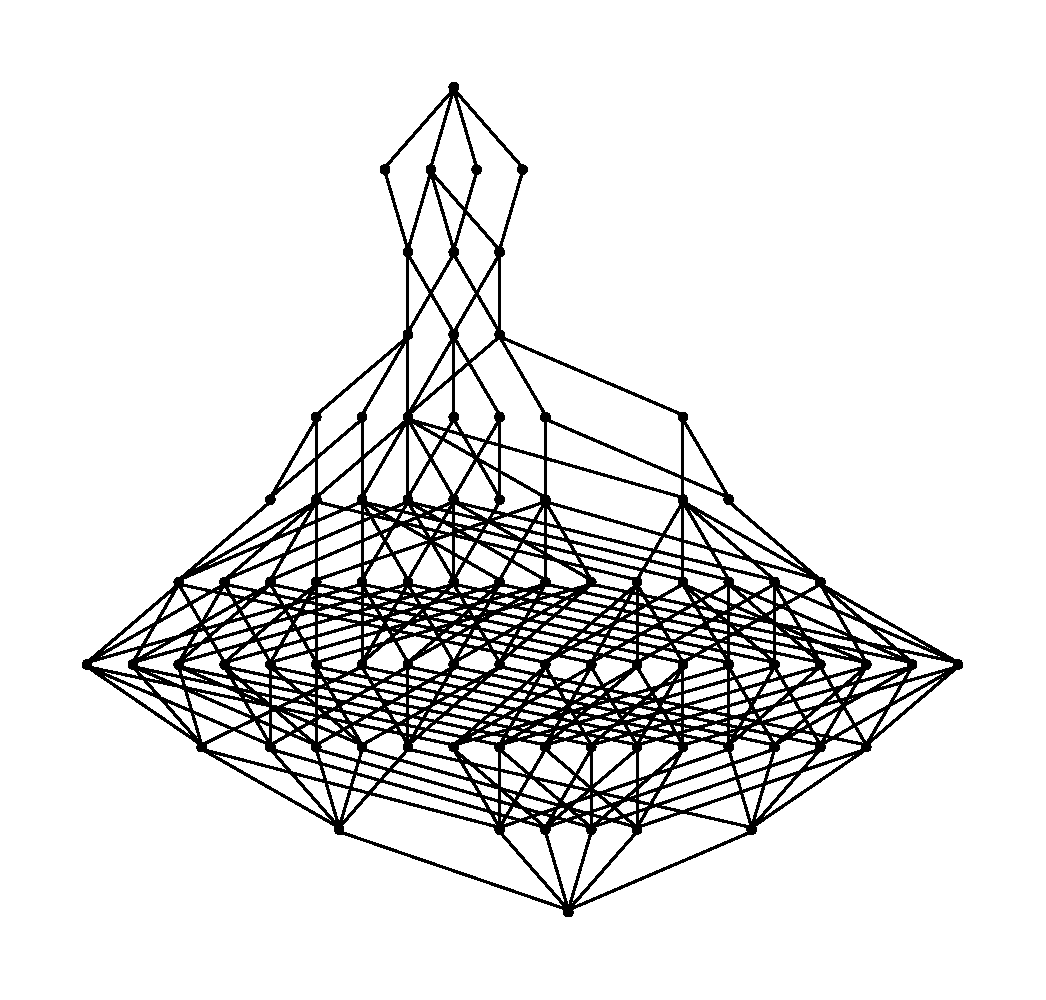
\includegraphics[width=\textwidth]{pics/ch-lattice/gossip3.pdf}
  \texttt{gap> Splash(DotString(LatticeOfCongruences(GossipMonoid(3))));}
  \caption[Congruence lattice of the Gossip monoid $G_3$]
  {Congruence lattice of the Gossip monoid $G_3$ \cite[\S2]{gossip}}
  \label{fig:g3-lattice}
\end{figure}

\begin{figure}[h]
  \centering
  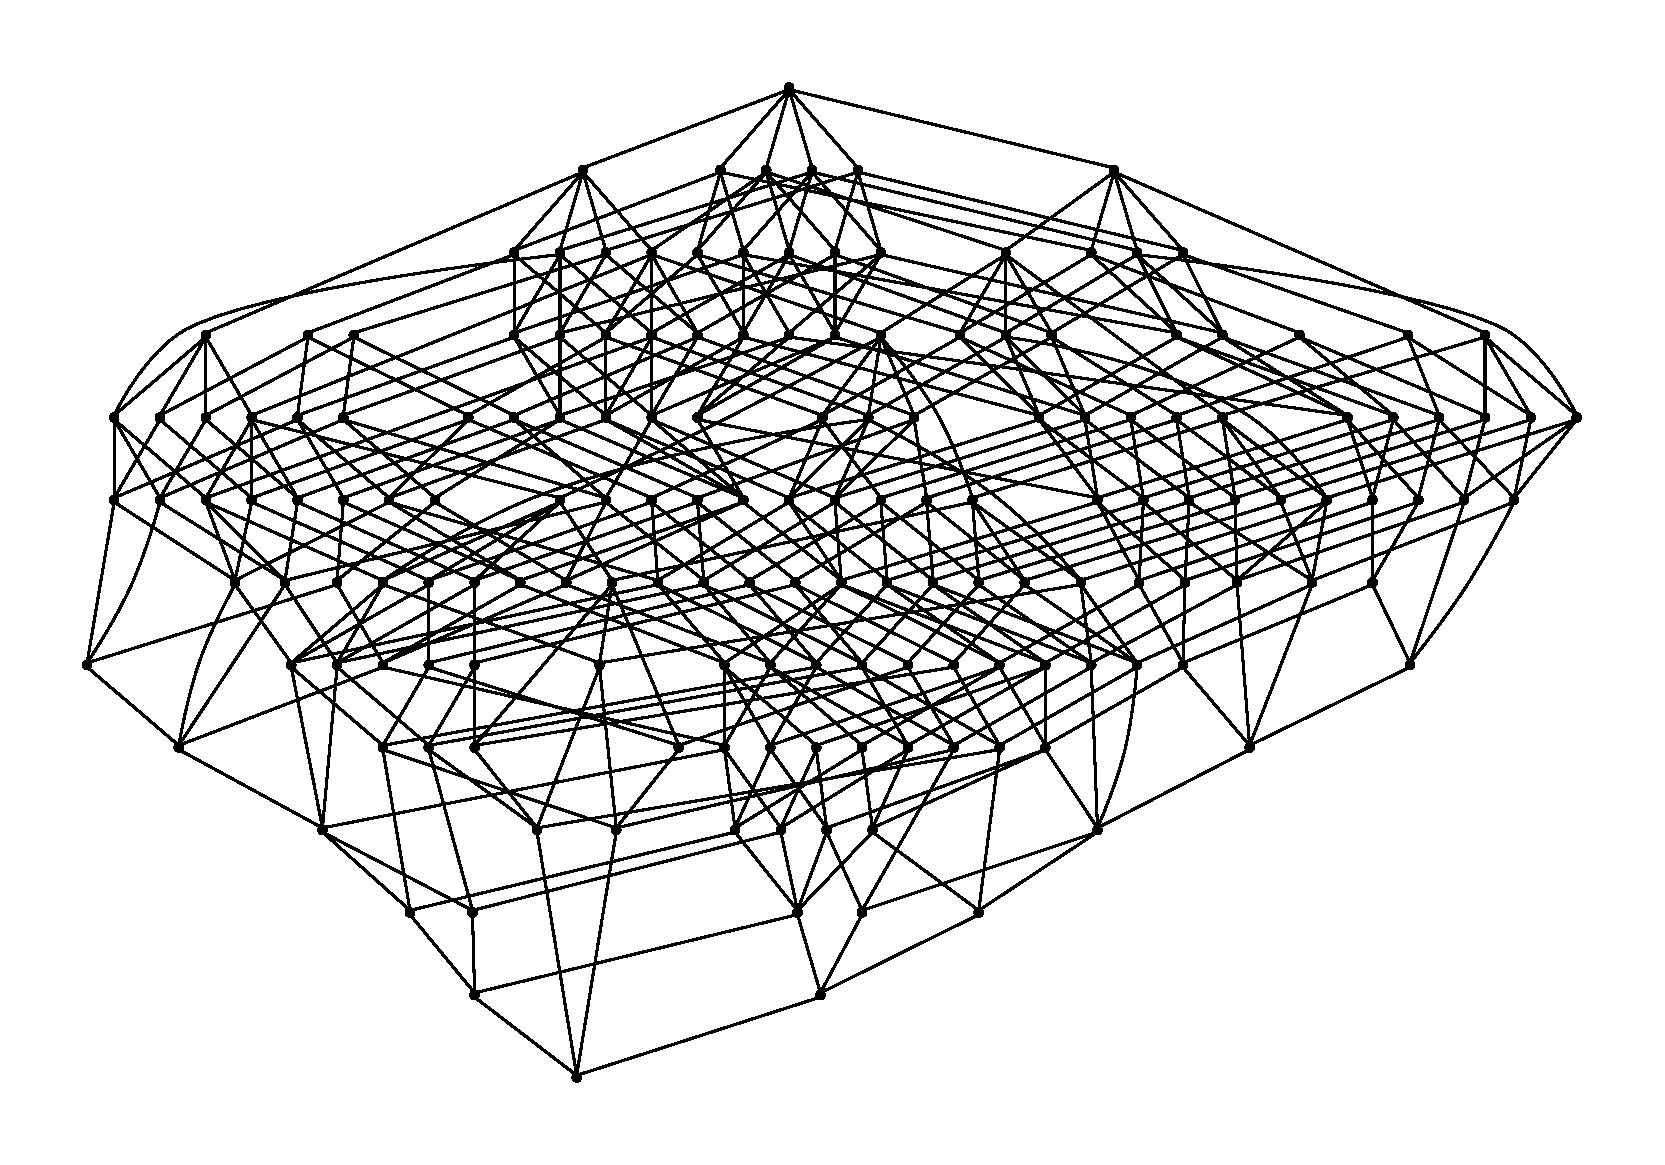
\includegraphics[width=\textwidth]{pics/ch-lattice/pbr1.pdf}
  \texttt{gap> Splash(DotString(LatticeOfCongruences(FullPBRMonoid(1))));}
  \caption[Congruence lattice of the full PBR monoid $\PBR_1$]
  {Congruence lattice of the full PBR monoid $\PBR_1$
    \cite[\S2.1]{diagram_semigroups}}
  \label{fig:pbr1-lattice}
\end{figure}

\begin{figure}[h]
  \centering
  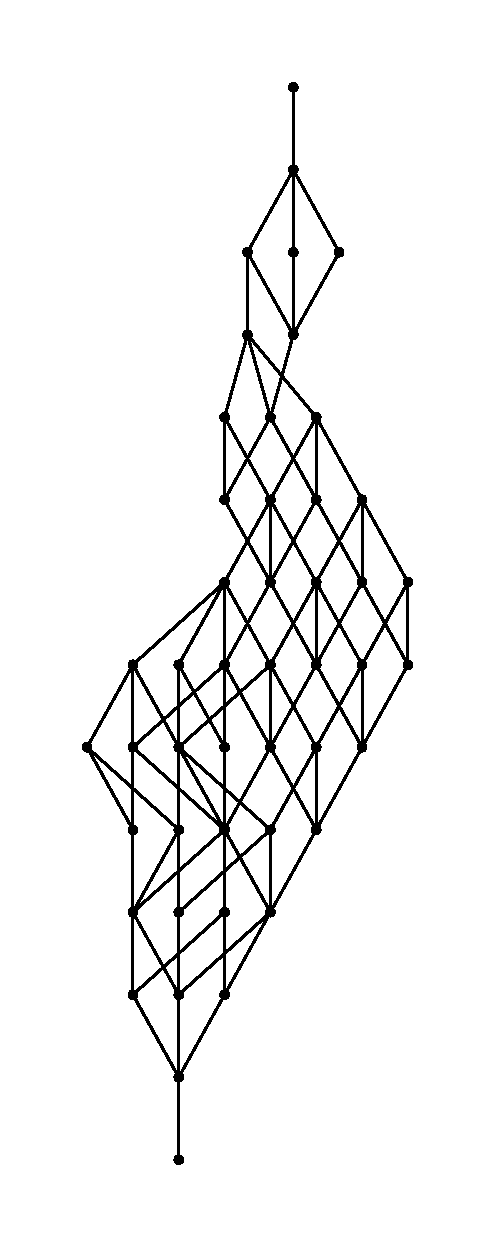
\includegraphics[height=0.9\textheight]{pics/ch-lattice/c2-wr-t3.pdf}
  \doublespacing
  \vspace{-1.5cm}
  \begin{align*}
    &\texttt{gap> C2 := Group((1, 2));;} \\
    &\texttt{gap> T3 := FullTransformationMonoid(3);;} \\
    &\texttt{gap> W := WreathProduct(C2, T3);;} \\
    &\texttt{gap> Splash(DotString(LatticeOfCongruences(W)));}
  \end{align*}
  \vspace{-1.0cm}
  \caption[Congruence lattice of the Wreath product $C_2 \wr \T_3$]
  {Congruence lattice of the Wreath product $C_2 \wr \T_3$
    \cite[\S10.1]{wreath}}
  \label{fig:c2-wr-t3-lattice}
\end{figure}

Since the algorithm described above was implemented in the Semigroups package
\cite{semigroups}, it has been possible to compute the congruence lattice of any
sufficiently small semigroup.  Part \ref{part:results} of this thesis examines
the congruence lattices of a variety of semigroups, and attempts to explain
their structure.  Many of these lattices were originally computed using
\textsc{PrincCongPoset} and \textsc{JoinClosure}.  After examining these
lattices, it was possible in some cases to classify the congruences of entire
infinite families of semigroups, with proofs that were independent of any
computer code (see, for example, Theorems \ref{thm:mn-congs} and
\ref{thm:dkstar-congs}).  In others it was possible at least to produce
conjectures about families of semigroups, and to prove them for small cases (see
Conjectures \ref{conj:not-cong-full} and \ref{conj:cong-nearfull-7}).
